\documentclass[10pt,a4paper]{article}
\usepackage[utf8]{inputenc}
\usepackage{amsmath}
\usepackage{amsfonts}
\usepackage{amssymb}
\usepackage{graphicx}

\title{Transfer Learning for the Equivariant Prediction of Tensorial Properties in Material Systems}
\author{}
\begin{document}
\maketitle

\section{Introduction}




\subsection{Motivation for Transfer Learning of Tensors}

a

\subsection{Motivation/Intro for Original Paper}
The elastic properties of a material system are important for many potential applications, and thus their efficient and accurate prediction is an imperative task. 

One of the simplest models for the elastic deformation of a 3-dimensional solid is a generalization of Hooke's law, and corresponds to a linear relationship between applied forces and resulting strain (or vice versa). In such a linear   elastic model for a solid, the material's elastic properties are all encoded in a rank-4 \textit{elasticity tensor}, or for simplicity, it's \textit{elastic tensor}. Note that component-wise descriptions of a material's elastic tensor necessarily depend on a chosen coordinate system.

However, modern machine learning methods applied to the prediction of physical properties from encoded material systems often use representations and, correspondingly, network structures that are invariant under coordinate transformations. This poses a problem for tasks related to coordinate system-dependent quantities, as is the case for the elastic tensor.

Newer, $SO(3)$ equivariant models have recently been applied to the prediction of previous set of invariant physical quantities, despite being based on a representation space that might be used to encode higher-order geometrical information (that is, rotationally equivariant quantities).
 
In this work, we investigate the link between symmetric tensors and spherical harmonics (the irreducible representations of $SO(3)$) to the end of predicting a rotationally equivariant quantity, i.e. the elastic tensor of a material.

This approach greatly simplifies the prediction of elasticity data from a given material system, without specific need for considerations of different stresses and resulting strains, or the Strain-Elastic Density (as in StrainNet).

Below, we first introduce the concept of an equivariant network before presenting the relevant equivariant network for our application, defined with respect to the special Euclidean group in three dimensions $SE(3)$. Then, we'll present in some generality the link between tensors and spherical harmonics, specifically symmetric tensors. To aid such spherical harmonic decompositions, we then present the Young decomposition of a tensor which allows one to represent an arbitrary tensor as a collection of (in general, different rank) symmetric tensors. And finally, we show how all this may be used to equivariantly predict elastic tensors of arbitrary crystalline systems by way of $SE(3)$ equivariant networks.

\section{Equivariant Networks}
Suppose we are given some function $f:X\rightarrow Y$ and some symmetry group $G$ with group elements having representations acting on the domain $X$ and codomain $Y$. An \textit{equivariant function} $f$ is one which preserves the action of group elements operating on the input space, so that it satisfies the following relation:
$$
\quad\quad\quad f\big(\rho_X(g)x\big) = \rho_Y(g) f(x) \quad\quad\quad \forall g\in G, \ x\in X
$$
In a certain sense then, equivariant functions 'commute' with representations of group elements in their input and output spaces (though commute isn't exactly the right term if $X\neq Y$).

Note that invariance under some group is a special case of equivariance (where all it's corresponding group element's representations are just the identity).


Equivariant networks, in the context of machine learning, generally refer to neural networks with convolutional operators that are equivariant maps under some symmetry group (acting on the representation space). Since neural networks are typically composed layer-wise by consecutive application of layer-to-layer transition maps acting on hidden representation spaces, to construct an equivariant network, we need a set of equivariant transition maps to compose our network.

One such equivariant map is \textit{group equivariant correlation}, defined as:
$$
\big[f\star \psi \big](g) = \sum_{h\in G}\sum_K f_K(h)\psi_{K}(g^{-1}h)
$$
where $K$ are the channels from the previous layer's representation space, and $h,g$ are group elements of $G$ (the group for which the correlation function is equivariant). Note that this function (group equivariant correlation) takes as input a group element $g$ from the underlying symmetry group, so that the output layer's representation space will have features associated with each group element (as opposed to input channel features, i.e. pixel indices).


Such trainable, equivariant correlation functions may then be taken as one of the basic building blocks of a group equivariant network, in addition to the usual pooling and activation functions (which are themselves equivariant). These building blocks thus give us a concrete way to construct an equivariant network from some symmetry group.

Below, we'll consider two examples of such group equivariant models of particulat importance to the field of machine learning in the avenue of material's science: graph neural networks, and $SE(3)$ networks.

\subsection{Graph Neural Networks}


However, graphs representing physical systems (with purely scalar features) are also invariant under rotation, and this may be a nuisance in the case of coordinate-basis dependent prediction tasks. Consider this, a rotationally invariant network cannot be trained to learn any basis dependent physical quantity, since it itself is invariant under rotations and thus should only predict the same value for all rotated inputs.

Modern equivariant networks amend this issue by further associating hidden representations with irreducible representations of the group for each element. In the case of SO(3), these hidden representations are the harmonics. This results in a set of rotationally equivariant features (up to some maximum order) for each object of interest.


\subsection{SE(3) Equivariant Networks}
Let us now consider a specific implementation of an equivariant network: one specified by the special Euclidean group, SE(3). $SE(3)$ may be decomposed into a semidirect product of two subgroups $\mathbb{R}^3\rtimes SO(3)$. Where $\mathbb{R}^3$ is the translational subgroup of dimension 3; and $SO(3)$ is the special orthogonal group of dimension 3. $\mathbb{R}^3$ accounts for the translational movement of a given coordinate system's origin; whereas $SO(3)$ accounts for rigid rotations of the coordinate axes.

This group has great significance in the description of physical quantities. A quantity described relative to some coordinate system will generally transform as a tensor. This tensor is a map in a tensor product space formed by copies of $SE(3)$ or $SO(3)$.

For such models, we construct a graph representing the input data, and associate with each graph feature of interest (e.g. nodes, edge) a set of spherical harmonics up to some rotational order (analogous to a truncated multi-pole expansion).

The graph structure results in translational invariance under $\mathbb{R}^3$, a property often desired in physical quantity prediction. 

\subsection{$SE(3)$ Hidden Representations}
The representations of elements of the graph themselves are associated with analagous harmonics.

\subsection{$SE(3)$ Equivariant Convolution}

\subsection{Pooling}
Most all pooling functions are inherently equivariant. Summation over channels, respecting $\ell$ and $m$ values, is equivariant, as is maximum or minimum pooling of the same form.

\section{Spherical Harmonic Decomposition of a Tensor}
The spherical harmonic decomposition of a tensor is a partitioning into a set of disjoint subspaces $\mathcal{H}^{(n)}$ that are invariant under the action of the special orthogonal group $SO(3)$. 

Since $SO(3)$ is a subgroup of the general linear group $GL(3)$, we may apply the decomposition techniques of $GL(3)$ (and the symmetric group $S$, by way of the Schur-Weyl duality), namely Young diagrams. Such a $GL(3) $ decomposition returns a disjoint set of tensor spaces with equal rank and different, fixed symmetries.  


In $SO(3)$, we also may define a metric on the vector space, and thus have an invariant metric tensor $g_{ij}$ available; as well as a definable orientation, or volume element, resulting in an invariant totally anti-symmetric tensor $\epsilon^{ijk}$. These invariant tensors allow us to construct lower-rank $SO(3)$ tensor invariants of arbitrary higher-rank tensors by way of contractions with $g$ and $\epsilon$.

By means of the Young decomposition of $GL(3)$, and the further decompositions of $SO(3)$ by contractions with the invariant tensors $g$ and $\epsilon$, we may express an arbitrary rank tensor in terms of a set of variable-rank, invariant symmetric tensor spaces.

There then is a clear correspondence between symmetric tensor spaces and harmonic tensor spaces, a la tensor-valued spherical harmonics \cite{harmonictensors}.

To construct a spherical harmonic decomposition of a




The space formed by the solutions to the $n$-th rank tensorial form of Laplace's equation is generally referred to as the harmonic tensor space of rank $n$, $\mathcal{H}^{(n)}$, and is isomorphic to the space of traceless symmetric tensors of rank $n$, $
\mathcal{S}^{(n)}$.

\subsection{Motivational Example: Multipole Expansions}
Recall that a function $f(\theta,\phi)$, dependent only on angular parameters, has an expansion in terms of (scalar-valued) spherical harmonic functions:
$$
f(\theta,\phi)=\sum_{\ell=0}^{...}\sum_{m=-\ell}^{\ell}c_{\ell}^m Y_{\ell}^m(\theta,\phi)
$$
\begin{center}
with
\end{center}
$$
Y_{\ell}^m(\theta,\phi) = \sqrt{\frac{(2\ell+1)}{4\pi}\frac{(\ell - m)!}{(\ell+m)!}}P_{\ell}^m (\cos \theta)e^{im\phi}
$$
where $P^{m}_{\ell}$ are the associated Legendre polynomials, and we neglect the "Condon-Shortley" phase of $(-1)^m$ since it will be unnecessary in our applications. 

If we then define the unit vector $\hat{n} = x_+\hat{j}^++ x_0 \hat{z} + x_-\hat{j}^-$, we may rewrite the above expansion in terms of the vector components $n_i$:
$$
f(\theta,\phi) = \tilde{c} + \tilde{c}_i n_i + \tilde{c}_{ij}n_in_j + \tilde{c}_{ijk}n_in_jn_k+ ...
$$
Note that we may choose any basis to expand in this. However, if we choose the coefficients to be in the $J_z$ basis, the coefficients $c_{\ell}^m$ here correspond to the coefficients in the previous spherical harmonic expansion via Clebsch-Gordon coefficients (take $\hat{j}^{\pm}=Y_{\ell=1}^{m=\pm 1}$ and expand the above relation). 

These forms of expansion will be developed in parallel in the case of tensor-valued functions to arrive at a spherical harmonic expansion of tensors. But first, we introduce the spherical harmonic tensors, which form a natural basis for symmetric tensor spaces.

\subsection{Spherical Harmonic Tensors}
Just as there are a set of scalar-valued functions spanning the space of solutions to the scalar valued Laplace equation, there are tensor-valued functions of a similar charachter associated with the tensor-valued Laplace equation:
$$
\nabla^2 \mathbf{L} = 0
$$

\section{Elastic Tensors}
Suppose we would like to model the deformation of some volume of a homogeneous material under some applied set of (small) forces acting upon it's surface.

The simplest model of such a scenario is a generalization of Hooke's law to continuum mechanics, where we may consider the above scenario now in regards to an infinitesimally small cube of the material. 

The Cauchy stress tensor then describes the sheer and compressive (or expansive) forces on each face $\epsilon$. And the symmetric components of the material's resulting deformation then correspond to the material's strain $\tau$.

The elasticity (or simply, elastic) tensor $C$ of a material relates it's Cauchy strain  to some small applied stress . This may be described, component-wise, as the linear relation below:
$$
\epsilon_{ij}=C_{ijkl}\tau_{kl}
$$
As should be clear by the number of indices, the elastic tensor is a fourth rank tensor. The symmetries of the elastic tensor are discussed below, as they are relevant for our application. However, it is worth noting here that the total number of independent components of the elastic tensor is 21 in general.


\subsection{Symmetries of the Elastic Tensor}

The elastic tensor has several symmetries, but is not, in general, symmetric upon any swapping of indices. For general systems, $C$ satisfies the so-called 'minor symmetries' below:
$$
C_{ijkl}=C_{jikl}
$$

$$
C_{ijkl}=C_{ijlk}
$$
resulting from the symmetry of the strain and stress tensors ($\tau_{ij}=\tau_{ji}$ and $\epsilon_{ij}=\epsilon_{ji}$) under the assumption of equilibrium. This reduces the number of independent components from 81 to 36.

Furthermore, for conservative systems in which the elastic deformation is describable in terms of some potential energy function (and which we shall henceforth assume for our application), $C$ has the additional 'major symmetry':
$$
C_{ijkl}=C_{klij}
$$
This further reduces the number of independent components from 36 (from the minor symmetries) to 21 in total.


Following the approach in Backus, the Elastic tensor of a material may always be broken into a symmetric tensor $S$ and an asymmetric (note, not \textit{anti}symmetric) tensor $A$, defined by:

$$
S_{ijkl}=\frac{1}{3}\big( C_{ijkl} + C_{ikjl} + C_{klij} \big)
$$
$$
A_{ijkl} = \frac{1}{3}\big( 2C_{ijkl} -C_{ikjl} -C_{klij}  \big)
$$
\begin{center}
so that:
\end{center}
$$
C_{ijkl} = S_{ijkl} + A_{ijkl}
$$

Note that $S$ then is symmetric under any permutation of it's indices, whereas $A$ is not. In fact, if we examine the Young diagrams of a fourth rank tensor, as below: 

\begin{center}
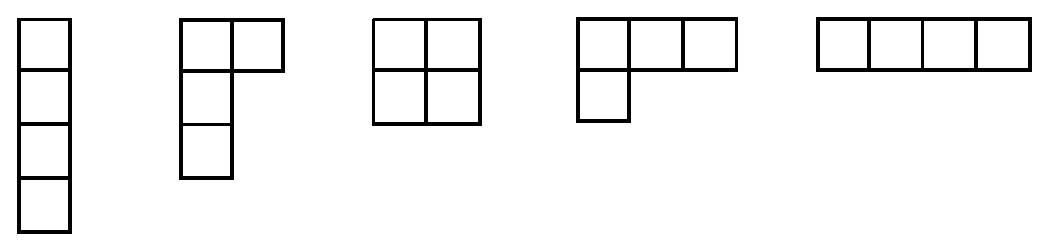
\includegraphics[scale=0.7]{rank4_young.pdf}
\end{center}

We can immediatley notice that the symmetries of $C$ require that all but the totally symmetric tensor $S$ and one mixed symmetry tensor $A$ (with symmetries $S(ij)S(kl)A(ij)A(kl)$) must vanish. Thus, $A$ is exactly the tensor symmetric under permutation of $i,j$ and $k,l$ but antisymmetric under any other exchange $i,k$ and $j,l$.
\begin{center}
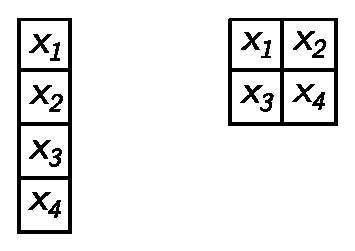
\includegraphics[scale=0.7]{elastic_young.pdf}
\end{center}
This fourth rank mixed-symmetry tensor $A$ may be decomposed into a symmetric rank-two tensor $s$ and a scalar $a$ according to the relations of Backus:
$$
A_{ijkl}^{(0)}=s\big(\delta_{ij}\delta_{kl}-\frac{1}{2}\delta_{ik}\delta_{jl}-\frac{1}{2}\delta_{il}\delta_{kj}\big)
$$
$$
A_{ijkl}^{(2)}=\delta_{ij}s_{kl} + \delta_{kl}s_{ij} - \frac{1}{2}\delta_{ik}s_{jl}- \frac{1}{2}\delta_{jl}s_{ik}- \frac{1}{2}\delta_{il}s_{jk}- \frac{1}{2}\delta_{jk}s_{il}
$$

\subsection{Harmonic Decomposition of the Elastic Tensor}

Since we now have three symmetric tensors (the rank-four $S$, rank-two $s$, and rank-zero $a$) describing the entire space of elastic tensors, we may form a harmonic decompostion of the elastic tensor space.

The rank-four symmetric tensor $S$ has a decomposition in the space $\mathcal{H}^{(4)}\oplus\mathcal{H}^{(2)}\oplus\mathcal{H}^{(0)}$ with 15 components; whereas the aforementioned breakdown of $A$ results in an apparent decomposition in the space $\mathcal{H}^{(2)}\oplus\mathcal{H}^{(0)}$ with 6 components: five for $s$ and one for $a$. This accounts for all 21 independent components of the elastic tensor.

The relations between harmonic components $h_{l}^{m\ (p)}$ of $C$ and real-space components $C_{ijkl}$ is most easily seen in the $J_z$ basis defined by the following transformation from Cartesian space (as in Mochizuki):

$$
x_{+} = -\frac{1}{\sqrt{2}} (x + i y) = \sqrt{4	\pi} Y_{1}^1
$$
$$
x_{0} = z = \sqrt{4	\pi} Y_{1}^0
$$
$$
x_{-} = \frac{1}{\sqrt{2}} (x - i y) = \sqrt{4	\pi} Y_{1}^{-1}
$$
Note that in this basis, the components of a vector correspond to the $\ell=1$ rotational order tensorial spherical harmonics evaluated for the vector $\vec{n} = \sum_i x_i e_i$. Thus, this basis effectively corresponds to the harmonic decomposition of a vector (in the space $\mathcal{H}^{(1)}$). Vectors should always have a harmonic decomposition since they are trivially symmetric.

In the $J_z$ basis, the coefficients of a vector correspond to it's \textit{spherical harmonic decomposition}. Perhaps the clearest way to see this correspondence is to note the similarity between the polynomial forms of the $\ell=0$ spherical harmonics and the transformation defined above.

The $J_z$ basis gives us a very natural way to make a correspondence between real-space tensor components and harmonic coefficients via an expansion with Clebsch-Gordan coefficients. Recall the following relation between (tensor) products of spherical harmonics, as is commonly used in addition of angular momentum:
$$
Y_{l_1}^{m_1}Y_{l_2}^{m_2} = \sum_{L = |l_1-l_2|}^{l_1+l_2}\sum_{M=|m_1-m_2|}^{m_1+m_2}c^{L0}_{l_1 0 l_2 0}c^{LM}_{l_1 m_1 l_2 m_2}Y_L^M
$$
where the $c$ are Clebsch-Gordan coefficients.
\subsubsection{Harmonic Decomposition of $A$}
Using the relations of Backus we can provide a set of harmonic coefficients describing $s$ and $s_{ij}$ to provide a harmonic decomposition of $A_{ijkl}$.

\subsubsection{Harmonic Decomposition of $S$}
The fully symmetric part $S$ of $C$ may be readily decomposed into it's harmonic components. The coefficients for such a transformation are given in \ref{fig:e-s-coeff}.

\begin{figure}

\begin{tabular}{c|rrrrrr}
 & $a_{000}$ & $a_{0\mp\pm}$ & $a_{00\pm}$ & $a_{\pm\mp\pm}$  & $a_{0\pm\pm}$ & $a_{\pm\pm\pm}$ \\
 \hline \\ 
$y_1^0$  & $3$ & $-6$ \\
$y_3^0$  & $\frac{15}{7}$ & $-\frac{5}{7}$ \\
$y_1^{\pm 1}$  &  & & $\sqrt{\frac{3}{2}}$ & $-2\sqrt{\frac{3}{2}}$\\
$y_3^{\pm 1}$  &  & & $2\sqrt{\frac{3}{2}}$ & $\sqrt{\frac{3}{2}}$\\
$y_3^{\pm 2}$  &  & & & & $\sqrt{\frac{15}{2}}$\\
$y_3^{\pm 3}$  &  & & & & & $\sqrt{\frac{5}{2}}$\\

 $y_3^{\pm 2}$  &  & & & & $\sqrt{\frac{15}{2}}$\\

\label{fig:e-s-coeff}
\end{tabular}

\caption{Coefficients for transformation between spherical basis components $a_{\alpha\beta\gamma}$ and harmonic components $y^m_l$ for a rank-three symmetric tensor}
\end{figure}

\subsection{Real Harmonic Decomposition of the Elastic Tensor}
The above treatment utilized the canonical harmonic functions (that is, those spanning complex spaces), but the elastic tensor is necessarily real valued. In fact, the above treatment results in general in complex valued components that come in conjugate pairs so that $h_{\ell}^{m \ (p)}=(i^m h_{\ell}^{m \ (p)})^*$. This points to a simplified, real harmonic decomposition, where the real harmonics $Y_{\ell m}$ are defined in terms of the complex-valued, canonical harmonics $Y_{\ell}^m$:
$$
Y_{\ell m }=
\begin{cases}
\frac{i}{\sqrt{2}}\big(Y_{\ell}^{-|m|} - (-1)^m Y_{\ell}^{|m|} \big):\ \ m<0\\
\quad\quad\quad\quad Y_{\ell}^0:\quad\quad\quad\quad\quad\ \ \  \ m=0\\
\frac{1}{\sqrt{2}}\big(Y_{\ell}^{-|m|} + (-1)^m Y_{\ell}^{|m|} \big):\ \ m>0\\
\end{cases}
$$



\section{Dielectric Tensors}

Dielectric tensors relate the applied electric field $E$ to the resulting electric displacement (in a material) $D$. Since $E$ and $D$ are vector fields, they're rank-one tensors and must be related by a rank-two tensor, namely the dielectric tensor $\varepsilon$:
$$
D_i=\varepsilon_{ij}E_j
$$
\subsection{Symmetries of the Dielectric Tensor}
The dielectric tensor is symmetric under permutation of it's indices. This leads to a straight-forward harmonic decomposition, formed most easily in the $J_z$ basis as

\section{Piezoelectric Tensors}
The piezoelectric strain constants $(d_{ijk})_{T}$ are defined (at constant temperature) by the thermodynamic relation:
$$
\big(d_{ijk}\big)_{T}=\left(\frac{\partial \epsilon_{ij}}{\partial E_k} \right)_{\sigma, T}
$$
where $\epsilon$ is the strain tensor, and the partial derivative is taken at constant stress $\sigma$ and temperature $T$.

These strain constants $d_{ijk}$ are related to the piezoelectric stress constants $e_{ijk}$ via the elastic $K$ according to:
$$
\big(e_{ijk}\big)_T=\big(d_{ilm}\big)\big(C_{ijkl}\big)_{E,T}
$$
\begin{center}
with $e_{ijk}$ defined as:
\end{center}
$$
\big(e_{ijk}\big)_{T}=\left(\frac{\partial D_{i}}{\partial \epsilon_{jk}} \right)_{\sigma, T}
$$
where $D$ is the resulting electric displacement vector in the material.

\subsection{Symmetries of the Piezoelectric Tensor}
The piezoelectric strain components $d_{ijk}$ are symmetric under $i,j$ due to the symmetry of the strain tensor $\epsilon_{ij}$, so that we have:
$$
d_{ijk}=d_{jik}
$$

The Young diagrams for a rank-three tensor are as follows:
\begin{center}
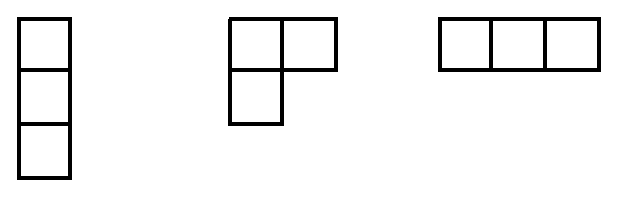
\includegraphics[scale=0.7]{youngdiagrams3.pdf}
\end{center}
according to the symmetry above, we can again see that all Young tableaux but the following will disappear:
\begin{center}
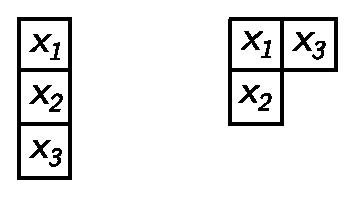
\includegraphics[scale=0.7]{piezo_young.pdf}
\end{center}
where the totally symmetric component tensor here we define as $S$ and the mixed symmetry component tensor we define $A$, so that we have the Young decomposition:
$$
d_{ijk} = S_{ijk}+A_{ijk}
$$
defined component-wise in terms of strain components:
\begin{align*}
S_{ijk}&=\frac{1}{3}\big(d_{ijk}+d_{jik}+d_{kji}\big)\\
A_{ijk}&=\frac{1}{3}\big(2d_{ijk}-d_{jik}-d_{kji}\big)\\
\end{align*}

\subsection{Harmonic Decomposition of the Piezoelectric Tensor}

The symmetric part $S$ is readily decomposed in the spherical bases into $\mathcal{H}^{(1)}\oplus \mathcal{H}^{(3)}$, with coefficients for the transformation given in TABLE.
\begin{figure}

\begin{tabular}{c|rrrrrr}
 & $a_{000}$ & $a_{0\mp\pm}$ & $a_{00\pm}$ & $a_{\pm\mp\pm}$  & $a_{0\pm\pm}$ & $a_{\pm\pm\pm}$ \\
 \hline \\ 
$y_1^0$  & $3$ & $-6$ \\
$y_3^0$  & $\frac{15}{7}$ & $-\frac{5}{7}$ \\
$y_1^{\pm 1}$  &  & & $\sqrt{\frac{3}{2}}$ & $-2\sqrt{\frac{3}{2}}$\\
$y_3^{\pm 1}$  &  & & $2\sqrt{\frac{3}{2}}$ & $\sqrt{\frac{3}{2}}$\\
$y_3^{\pm 2}$  &  & & & & $\sqrt{\frac{15}{2}}$\\
$y_3^{\pm 3}$  &  & & & & & $\sqrt{\frac{5}{2}}$\\

 $y_3^{\pm 2}$  &  & & & & $\sqrt{\frac{15}{2}}$\\

 
\end{tabular}

\caption{Coefficients for transformation between spherical basis components $a_{\alpha\beta\gamma}$ and harmonic components $y^m_l$ for a rank-three symmetric tensor}
\end{figure}

\nocite{*}




\bibliographystyle{annotate}
\bibliography{\jobname}

\end{document}
